\scanpage{14}\mspage{11.}
\reversemarginpar
% margin note written sideways
\margin{\figure{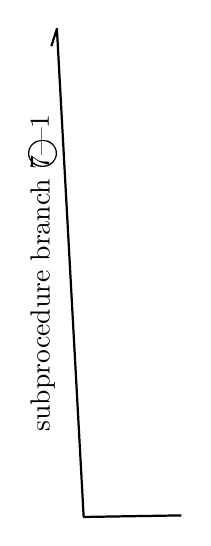
\begin{tikzpicture}[x=1cm,y=1cm]
\node[rotate=90,inner sep=1pt] at (0,-3.1) {subprocedure branch \textcircled{\unsure{7|1}}};
\draw[line width=.8pt,line join=round] (.10,-.22) -- (.17,0) -- (.51,-6.2) -- (1.75,-6.18);
\end{tikzpicture}}}%
If $a_{2,1}X^2+a_{4,3}X+a_{6,5}\equiv0$ has double root, then we can translate $x$ so that the root is $X\unsure{=|\equiv}0$, so that $\mathfrak p^4\mid a_4$ and $\mathfrak p^6\mid a_6$. Equation is now
\[
 y_3^2+\pi a_{1,1}x_3y_3+a_{3,3}y_3
 =\pi^3x_3^3\unsure{+|-}\pi^2a_{2,1}x_3^2+\pi^2a_{\unsure{1|4},4}x_3+a_{6,6}
 \tag*{\fbox{7.3}}
\]

If $Y^2+a_{3,3}\deleted{y}Y-a_{6,6}\equiv0$ has distinct roots, then
\[
 \unsure{\nu|v}=3,\quad\text{and}\quad c=\begin{cases}
 4&\text{if roots are in }k\\
 2&\text{if not}.
 \end{cases}
\]

If otherwise \unsure{....|...} etc. Keep going until the quadratic congruence which appears has distinct roots.... The process terminates, because the coefficients $a_3$, $a_4$, and $a_6$ are being made more and more highly divisible by $\mathfrak p$. Hence also $b_4$, $b_6$ and $b_8$, hence also $\Delta$. But $\Delta$ is fixed under all changes of coordinates (translations) involved. A crude estimate gives $\nu\leq\operatorname{ord}\Delta-3$ if I'm not mistaken.

\margin{(Branch 3 begins)}\textcircled{8} Suppose now $P(T)\equiv0$ has a triple root. We may assume the root is $T\equiv0$, so $\boxed{\mathfrak p^2\mid a_2,\ \mathfrak p^3\mid a_4,\ \text{and }\mathfrak p^4\mid a_6}$. The equation is
\[
 y_2^2+\pi a_{1,1}x_2y_2+a_{3,2}y_2
 =\pi^2x_2^3+\pi^2 a_{2,2}x_2^2+\pi a_{4,3}x_2+a_{6,4}
 \tag*{\fbox{8.1}}
\]
If $Y^2+a_{3,2}Y-a_{6,4}\equiv0$ has distinct roots, then Type $\mathrm{IV}^{*}$ and
\[
 f=v(\Delta)-6,\qquad c=\begin{cases}3&\text{if roots are in }k\\1&\text{if roots }\notin k.\end{cases}
\]

\margin{(Branch 3 continues)}\textcircled{9} Suppose $Y^2+a_{3,2}Y-a_{6,4}\equiv0$ has a double root. Then we can Assume it is $Y\unsure{=|\equiv}0$, so $\boxed{\mathfrak p^3\mid a_3,\ \mathfrak p^5\mid a_6}$. The equation is now
\[
 \pi y_3^2+\pi a_{1,1}x_2y_3+\pi a_{3,3}y_3
 =\pi x_2^3+\pi a_{2,2}x_2^{\unsure{2|7}}+a_{4,3}x_2+a_{6,5}
 \tag*{\fbox{9.1}}
\]
If $a_{4,3}\ne0$, i.e. if $\mathfrak p^4\nmid a_4$, then Type $\mathrm{III}^{*}$, and
\[
 f=v(\Delta)-7\qquad\text{and}\quad c=2
\]

\margin{(Branch 3 continues)}\textcircled{\scriptsize 10} Assume $\boxed{\mathfrak p^4\mid a_4}$. Then if $\mathfrak p^6\nmid a_6$ th\deleted{\unsure{a|e}}e type is $\mathrm{II}^{*}$ and
\[
 f=v(\Delta)-8\qquad\text{and}\quad c=1.
\]
\normalmarginpar

If $\mathfrak p^6\mid a_6$, original equation was not minimal. Start over with
\[
 y_3^2+a_{1,1}x_2y_3+a_{3,3}y_3=x_2^3+a_{2,2}x_2^2+a_{4,4}x_2+a_{6,6}\quad!
\]
% archive sheet number: 13
